\section{Fundamentals}

\begin{tabular}{|l|c|c|}
\hline \textbf{Description} & \textbf{Symbol} & \textbf{Unit} \\ 
\hline Free electric charge in the system & $Q$ & $C = As$ \\
\hline Volumetric free charge density & $\rho$ & $\frac{C}{m^3}$ \\
\hline Individual electric current flowing through the surface $S$ & $I_i$ & $A$ \\
\hline Magnetic flux through the surface $S$ & $\Phi$	& $Wb = Tm^2$\\
\hline Induced voltage along the closed loop $\delta S$ & $u_i$ & $V$ \\
\hline Electric current density & $\vec{J} = \sigma \vec{E}$ & $\frac{A}{m^2}$\\
\hline Electric flux density & $\vec{D} = \epsilon \vec{E}$ & $\frac{C}{m^2} = \frac{As}{m^2}$\\
\hline Electric field & $\vec{E} = \frac{\vec{D}}{\epsilon}$ & $\frac{V}{m}$\\
\hline Magnetic flux density & $\vec{B} = \mu \vec{H}$ & $T = \frac{Vs}{m^2}$\\
\hline Magnetic field & $\vec{H} = \frac{\vec{B}}{\mu}$ & $\frac{A}{m}$\\
\hline Electric permittivity & $\epsilon = \epsilon_0 \epsilon_r$ & $\epsilon_0 = 8.85 \cdot 10^{-12} \left[\frac{F}{m} = \frac{As}{Vm}\right]$\\
\hline Magnetic permeability & $\mu = \mu_0 \mu_r$ & $\mu_0 = 4\pi \cdot 10^{-7} \left[\frac{Tm}{A} = \frac{H}{m} = \frac{Vs}{Am}\right]$ \\
\hline 
\end{tabular} 

\textbf{\\ \\ Gradient\\ \\}
\begin{minipage}[lt]{5cm}
	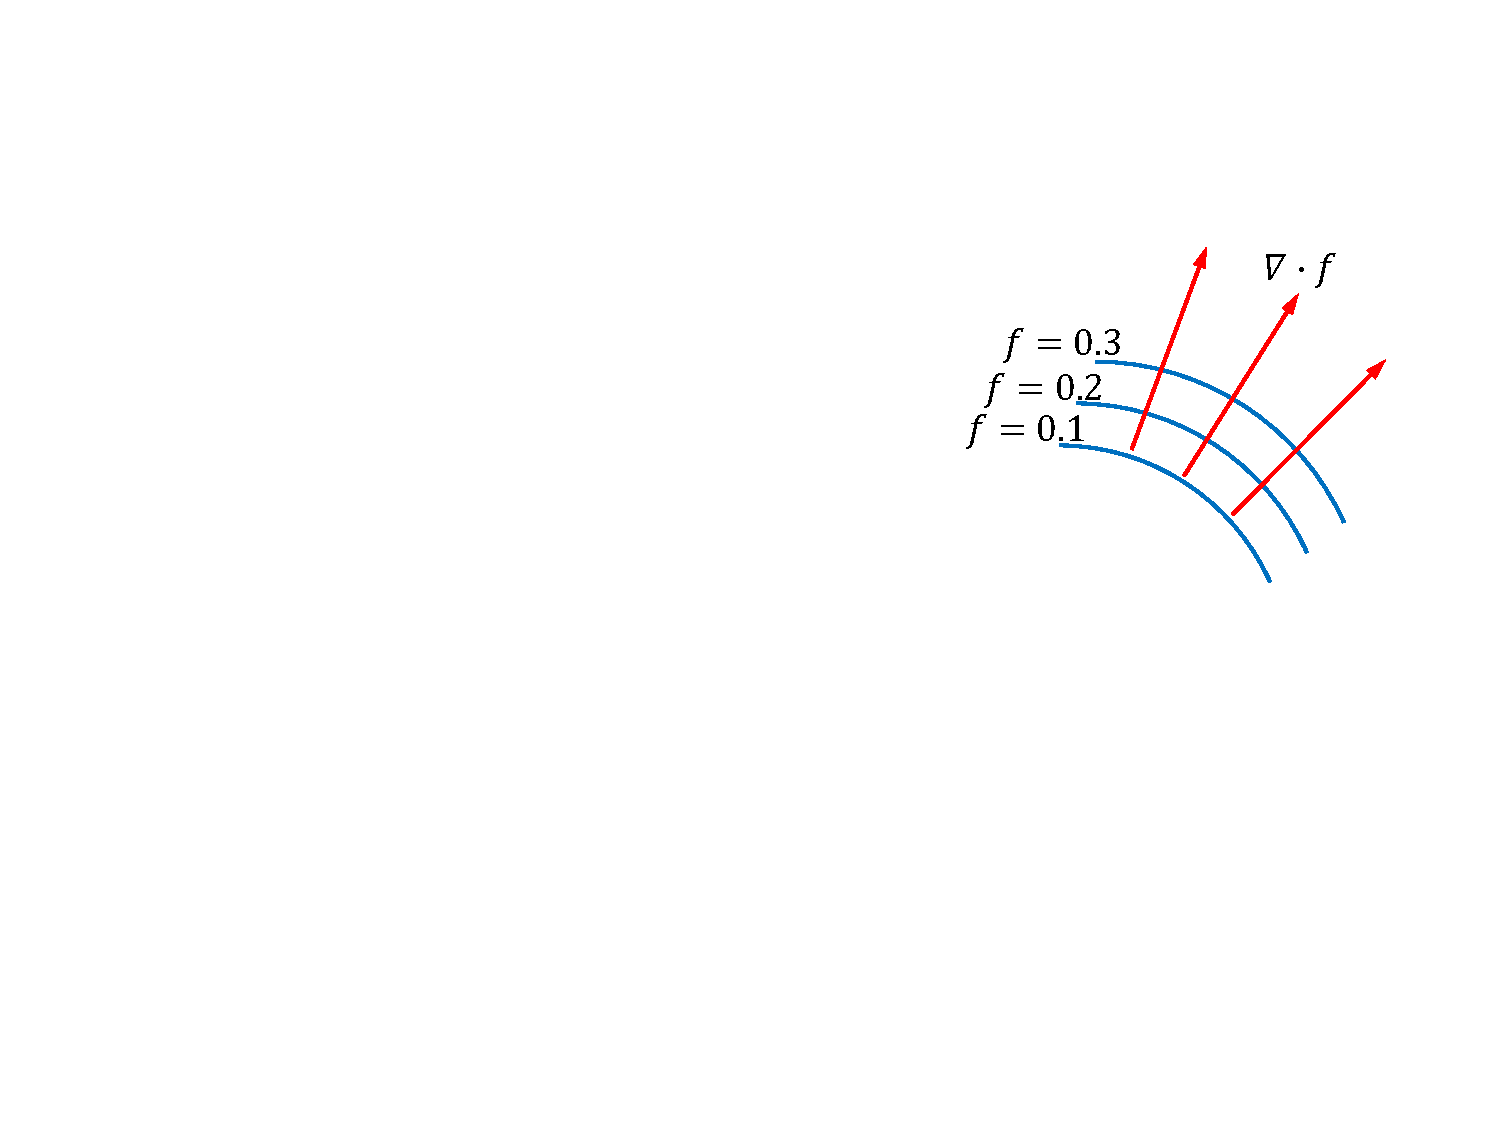
\includegraphics[width=.8\textwidth]{./images/Gradient.pdf}
\end{minipage}
\begin{minipage}[rt]{13cm}
	The gradient of a scalar field reveals the direction of the steepest ascent of the scalar function (perpendicular to the corresponding isolines of the function). \\ \\
	\begin{tabular}{ll}
		Scalar field: & $f = f\left(\vec{r}\right) = f\left(x,y,z\right)$ \\ 
		Gradient is a vector: & $grad f = \lim\limits_{diameter\left(D\right)\rightarrow 0} \frac{\oiint_{boundary\left(D\right)}f \cdot \vec{dA}}{measure\left(D\right)}, D\subseteq R^3 $\\
		Gradient in Cartesian coordinates: & $grad f = \frac{\partial f}{\partial x} \cdot \vec{e_x}+\frac{\partial f}{\partial y} \cdot \vec{e_y}+\frac{\partial f}{\partial z} \cdot \vec{e_z}$\\ 
		$\nabla$-operator (Nabla): & $\nabla = \frac{\partial}{\partial x} \cdot \vec{e_x}+\frac{\partial}{\partial y} \cdot \vec{e_y}+\frac{\partial}{\partial z} \cdot \vec{e_z}$\\
		Gradient and $\nabla$-operator: & $grad f = \nabla \cdot f$\\
	\end{tabular} 
\end{minipage}

\textbf{\\ \\ Divergence\\ \\}
\begin{minipage}[lt]{5cm}
	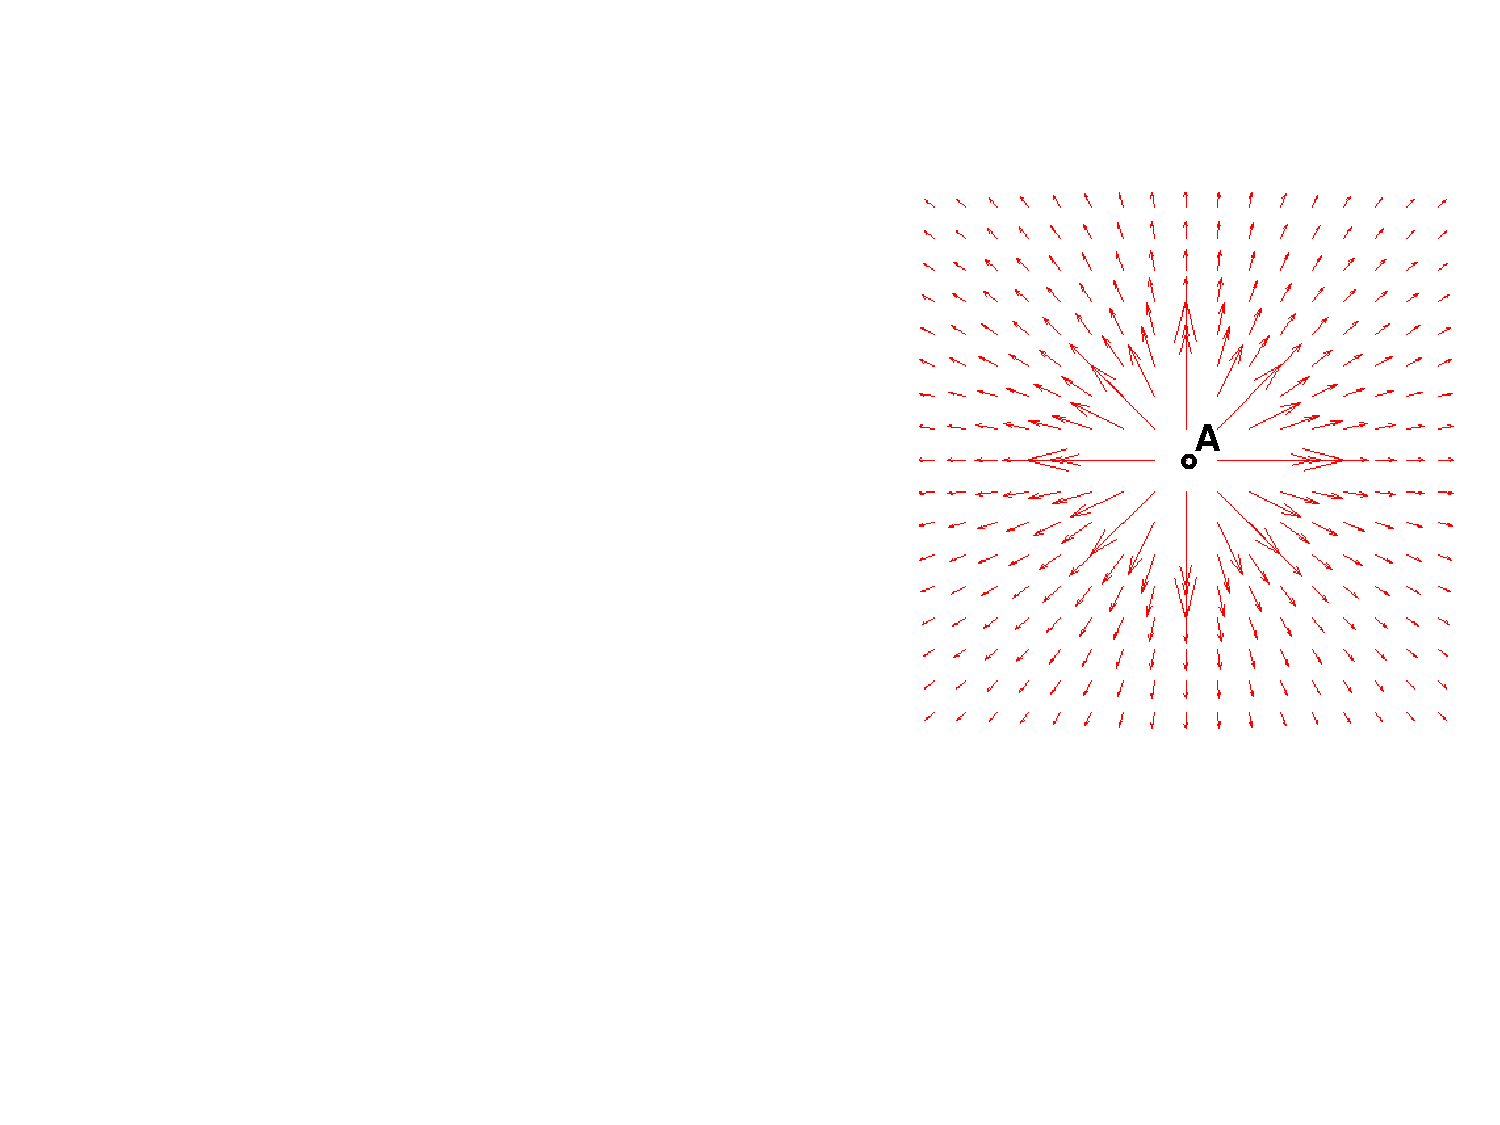
\includegraphics[width=.8\textwidth]{./images/Divergence.pdf}
\end{minipage}
\begin{minipage}[rt]{13cm}
	In the central point $A$ of this field distribution is: $div \vec{a} > 0$. Generally speaking, a positive or negative divergence reveals a field source or a field sink, respectively. \\ \\
	\begin{tabular}{ll}
		Vector field: & $\vec{a} = \vec{a}\left(\vec{r}\right) = \vec{a}\left(x,y,z\right)$\\
		Divergence is a scalar: & $div \vec{a} = \lim\limits_{diameter\left(D\right)\rightarrow 0} \frac{\oiint_{boundary\left(D\right)} \vec{a} \cdot \vec{dA}}{measure\left(D\right)}, D\subseteq R^3$\\
		Divergence in Cartesian coordinates: & $div \vec{a} = \frac{\partial a_x}{\partial x} + \frac{\partial a_y}{\partial y} + \frac{\partial a_z}{\partial z}$\\
		Divergence and $\nabla$-operator: & $div \vec{a} = \nabla \cdot \vec{a}$\\
	\end{tabular}
\end{minipage}

\textbf{\\ \\ Curl\\ \\}
\begin{minipage}[lt]{5cm}
	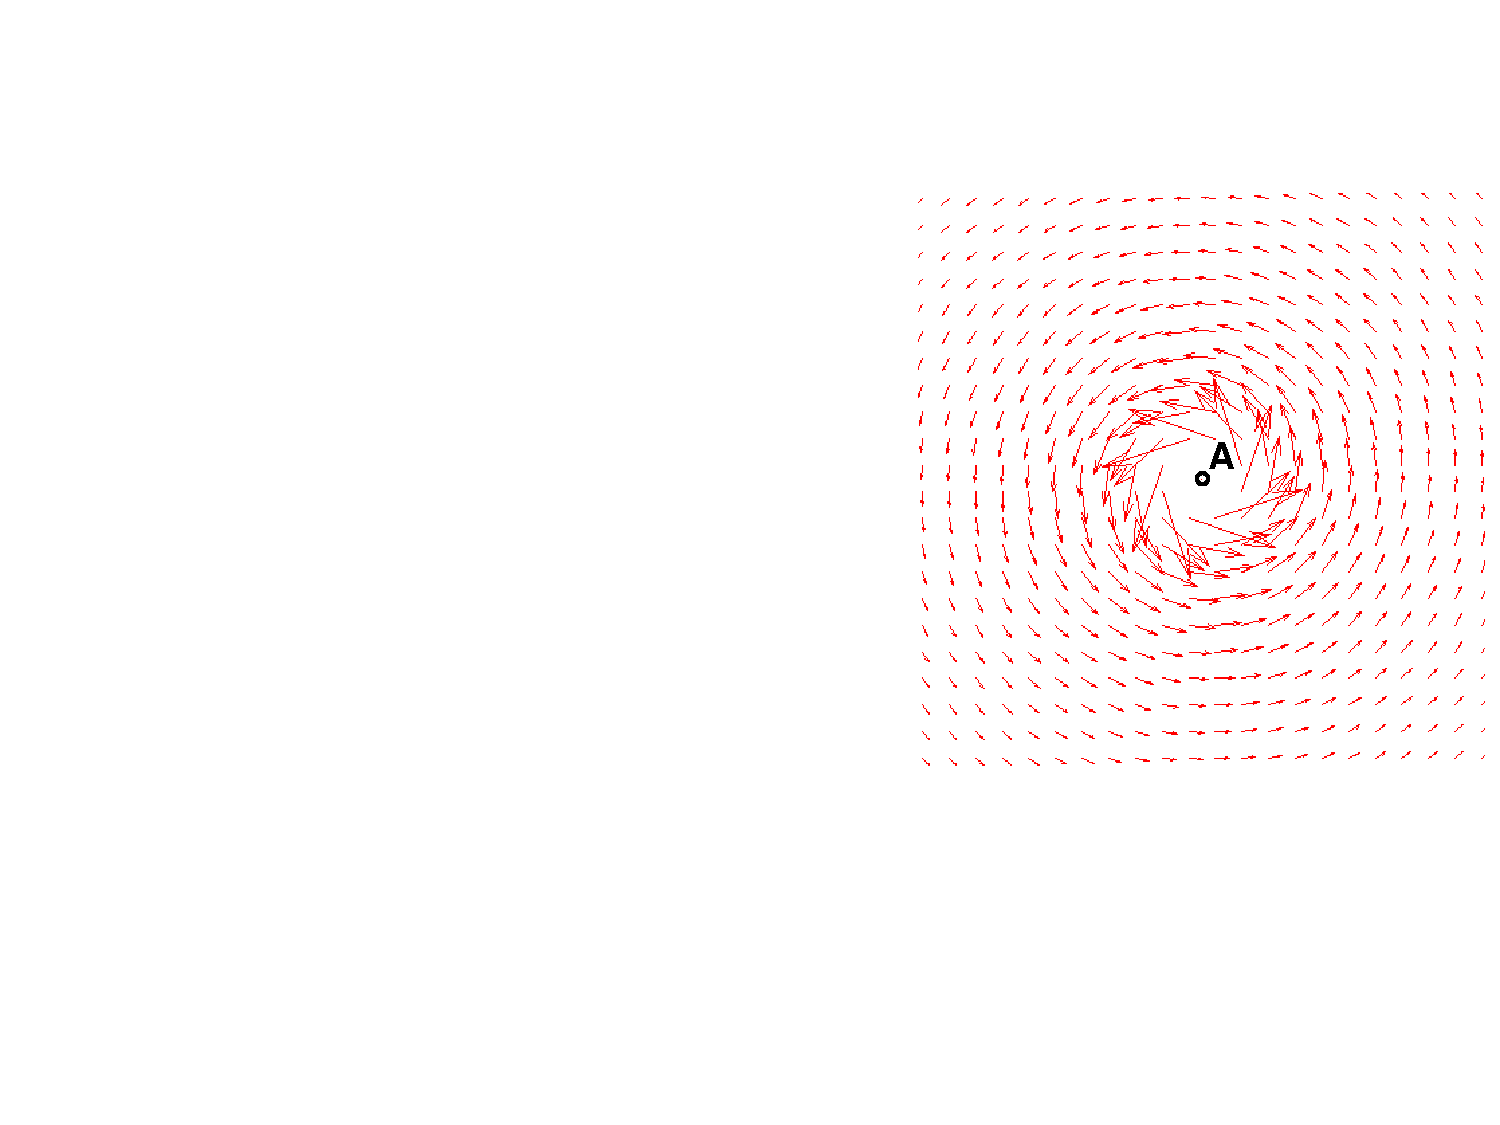
\includegraphics[width=.8\textwidth]{./images/Curl.pdf}
\end{minipage}
\begin{minipage}[rt]{13cm}
	In the central point $A$ of this field distribution is: $curl \vec{a} > 0$. Generally speaking non-zero curl reveals a rotational field character. (Curl looks what stays in this area).\\ \\
	\begin{tabular}{ll}
		Vector field: & $\vec{a} = \vec{a}\left(\vec{r}\right) = \vec{a}\left(x,y,z\right)$\\
		Curl is a vector: & $curl \vec{a} = \lim\limits_{diameter\left(D\right)\rightarrow 0} \frac{\oiint_{boundary\left(D\right)} \vec{dA} \times \vec{a}}{measure\left(D\right)}, D\subseteq R^3$\\
		Curl in Cartesian coordinates: & $curl \vec{a} = 
		\begin{vmatrix}
			\vec{e_x} & \vec{e_y} & \vec{e_z} \\
			\frac{\partial}{\partial x} & \frac{\partial}{\partial y} & \frac{\partial}{\partial z} \\
			a_x & a_y & a_z \\
		\end{vmatrix}$ {\tiny \texttt{other coordinates in Bronstein: P.719ff}}\\
		Curl and $\nabla$-operator: & $curl \vec{a} = \nabla \times \vec{a}$\\
	\end{tabular}
\end{minipage}

\textbf{\\ \\ Theorems\\}
\begin{tabular}{ll}
	Gauss theorem: & $\oiint\limits_{\left(\partial \Omega\right)} \vec{a} \cdot d\vec{S} = \iiint\limits_{\left(\Omega\right)} \nabla \cdot \vec{a}dV$\\
	Stokes theorem: & $\int\limits_{\left(\partial S\right)} \vec{a} \cdot d\vec{l} = \iint\limits_{\left(S\right)} \nabla \times \vec{a} \cdot d\vec{S}$\\
	Continuity equation: & $\oiint\limits_{\left(\partial \Omega\right)} \vec{J}\left(\vec{r}\right)\cdot d\vec{S}\left(\vec{r}\right) = -\frac{\partial Q}{\partial t} = -\iiint\limits_{\left(\Omega\right)} \frac{\partial \rho\left(\vec{r}\right)}{\partial t}dV\left(\vec{r}\right)$\\
\end{tabular}

\textbf{\\ \\ Rules \\}
\begin{tabular}{ll}
	Curl of a gradient is always equal to zero: & $\nabla \times \left(\nabla a\right) \equiv 0$ \\
	Divergence of a curl si always equal to zero: & $\nabla \cdot \left(\nabla \times \vec{a}\right) \equiv 0$\\
\end{tabular}